\chapter{Latent clusters}\label{ch:clusters}

With \opt{clusters(G)} the positions are drawn from a mixture of $G$ spherical normal distributions (Chapter~\ref{ch:model}): the actors fall into groups that lie together in the space. How many groups? The data do not say directly, and the number has to be chosen. This chapter fits clusters to Sampson's monastery~\cite{sampson1969}, 18 novice monks who named the fellow monks they liked, at several times. The anthropologist Sampson observed three factions during his stay, Loyal (7 monks), Turks (7) and Outcasts (4); the faction is stored as a node attribute, so the clusters can be compared with groups known from outside the model. \nwlsm{} fits a binary network, so we take the choices at the third time point and keep who was named at all:
\showlog{monks_data}
The network has 18 actors and 56 directed ties.

\section{The BIC of one model}\label{sec:bic}

\texttt{estat bic} computes the BIC of \latentnet{}'s \texttt{bic.ergmm()} for a binary network with the Euclidean distance, at the minimum Kullback--Leibler positions and effects:
\showlog{monks_bic}
The overall BIC is a sum of parts. The part for the ties given the positions ($Y$) is $-2$ times the log likelihood at the coefficients that maximise it for those positions and effects, plus the number of coefficients times the logarithm of the effective number of observations. \opt{effobs(ties | dyads | actors)} sets that number: the number of ties (the default), the number of dyads or the number of actors. The part for the positions ($Z$) is the normal log likelihood of the positions with the variance estimated from them (without clusters), or the log likelihood of a mixture of \opt{clusters()} spherical normal distributions with a free variance in each cluster, fitted to the positions by the EM algorithm, with the penalty of \latentnet{}. Each random effect adds a part. Smaller is better. As the help of \latentnet{} says, it is not certain that the BIC is appropriate for choosing the dimension or the random effects, or for comparing a clustered with an unclustered model.

\section{Comparing 0, 2, 3 and 4 clusters}\label{sec:select}

\texttt{nwlsmselect} fits the model once for every number of clusters in \opt{clusters()} (0 means no clusters; default \texttt{0 2 3 4}) with the same options and the same seed, and ranks the fits by BIC. \opt{refit} fits the best model again so that it is the active model; \opt{graph} draws the BIC. The table is returned in \texttt{r(table)} and the best number of clusters in \texttt{r(best)}.
\showlog{monks_select}
Read the parts. The part for the ties barely moves (180.0 without clusters, between 182.2 and 185.6 with them), and the mean log likelihood is about the same: clusters do not make the ties fit better. What changes is the part for the positions, which falls from 141.3 to 99.6 with three clusters. The BIC prefers three clusters over none (36.1 points) and over two (9.8), and four clusters are 7.5 behind. A difference of about 10 points is usually called strong, a difference below 2 or 3 hardly worth mentioning. The BIC is a rough guide.
\begin{figure}[ht]\centering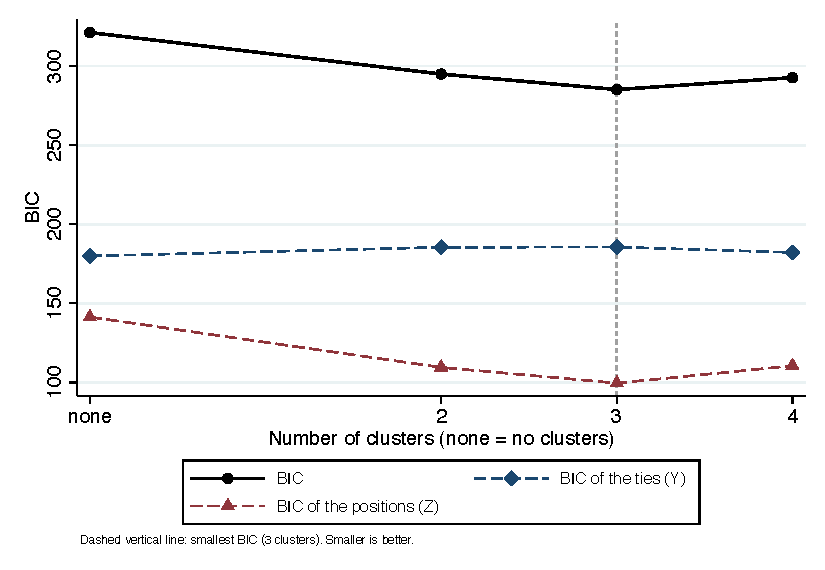
\includegraphics[width=0.85\textwidth]{fig/fig_monks_bic.pdf}
\caption{\texttt{nwlsmselect, graph}: the BIC of the monks network (solid), its part for the ties (dashed, $Y$) and for the positions (dashed, $Z$) against the number of clusters; the vertical dashed line marks the smallest BIC.}\end{figure}

\section{Do the clusters match the factions?}

The BIC tells which number of clusters describes the positions best; it does not tell that the clusters mean anything. \texttt{estat clusters} gives the classification and the posterior membership probabilities; with \opt{generate(stub)} they are stored in the variables \emph{stub}\texttt{\_class} and \emph{stub}\texttt{\_p1}, \emph{stub}\texttt{\_p2}, \dots{}
\showlog{monks_clusters}
The three clusters are the three factions, with no monk in the wrong place. The numbering of the clusters is arbitrary; only the grouping counts. The model has never seen the faction variable. Three monks have a largest membership probability below 0.8 and are the least certain.
\begin{figure}[ht]\centering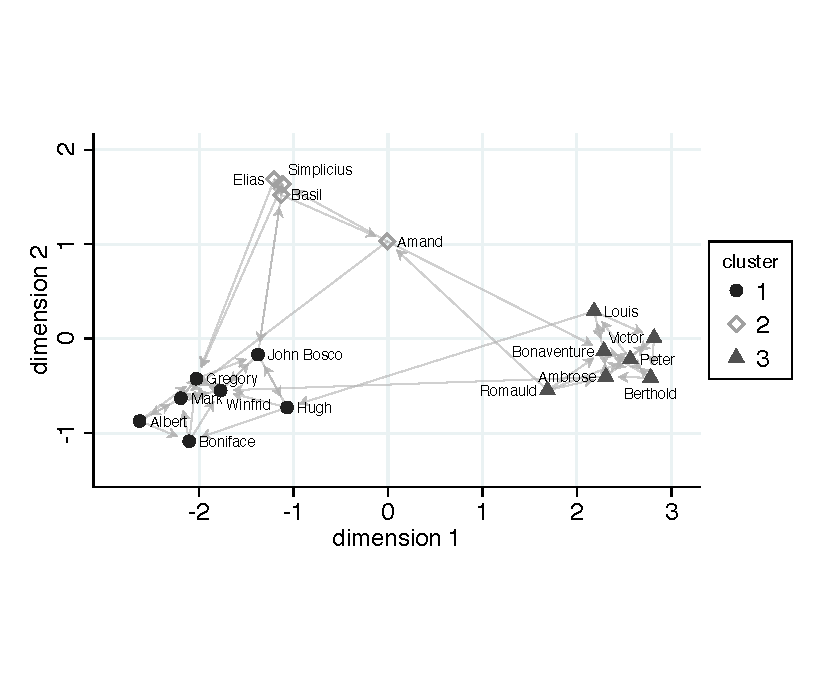
\includegraphics[width=0.85\textwidth]{fig/fig_monks_clusters.pdf}
\caption{The monks in the latent space (\texttt{nwlsmplot, clusters label(\_nwnode) colors(gray)}). The network is directed, so ties are drawn as arrows from the sender to the receiver.}\label{fig:clusters}\end{figure}
\begin{figure}[ht]\centering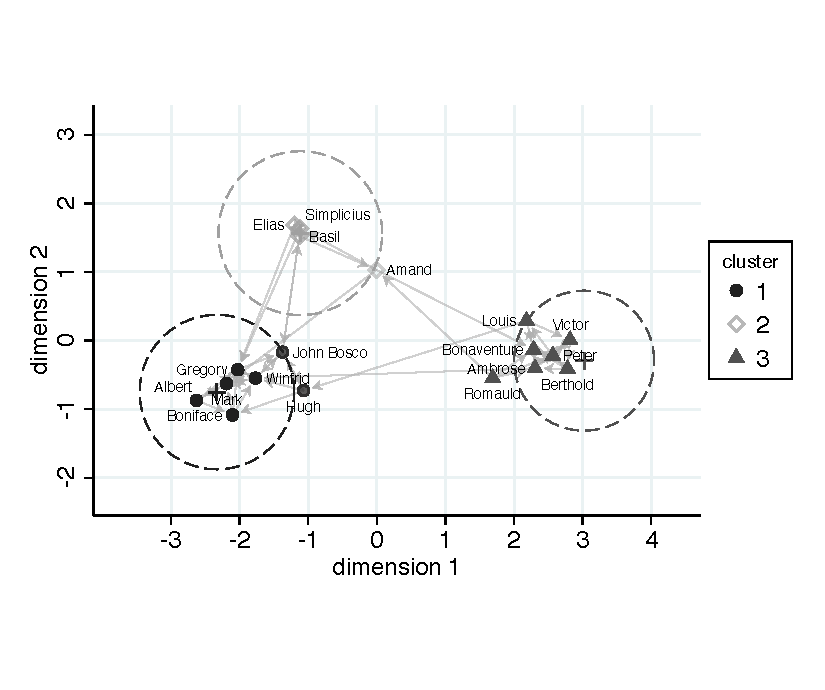
\includegraphics[width=0.85\textwidth]{fig/fig_monks_circles.pdf}
\caption{\texttt{nwlsmplot, clusters clustermeans circles certainty}: the mean of every cluster (a plus sign), a circle with the square root of the posterior mean variance of the cluster as radius, and the opacity of a marker by the largest posterior membership probability. Both axes have the same scale, so the circles are round.}\label{fig:circles}\end{figure}

\section{With random effects, and the effective number of observations}

With sender and receiver effects the picture is similar: three or four clusters, with a gap of 0.3 between them.
\showlog{monks_effects}
The overall BIC of the best model with random effects is 287.2, against 285.2 without them; the random effects add parts of their own ($-8.7$ for the senders, $27.0$ for the receivers). The number of starting points of the MKL fit is 4 here (Section~\ref{sec:deviations}); with a single start the numbers of this fit are the same. The BIC changes a little with the effective number of observations: 288.9 with the number of dyads (306), 286.0 with the number of actors (18), 287.2 with the number of ties (56).
